
\section{Das zentrale Dogma der Molekularbiologie}\label{sec:das-zentrale-dogma-der-molekularbiologie}

\begin{center}
    ``The central dogma states that information in nucleic acid can be perpetuated or transferred, but the transfer of
    information into protein is irreversible''
\end{center}

\begin{center}
    ``DNA macht RNA macht Protein''
\end{center}

\defin{dogma}

\begin{figure}[H]
    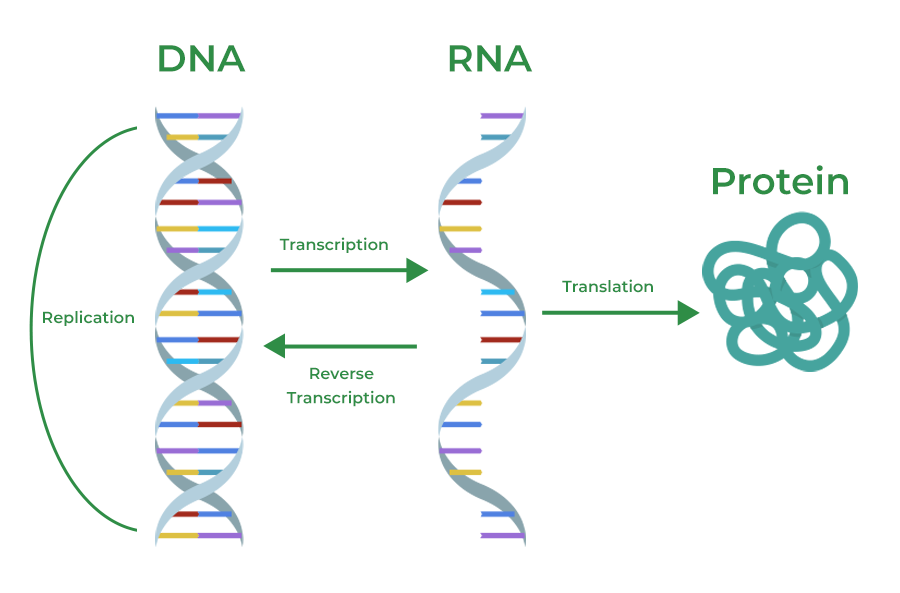
\includegraphics[width=\textwidth]{../eukgen/images/dogma}
    \caption{Code Sonne von \url{https://www.geeksforgeeks.org/biology/central-dogma-steps-guide/}}\label{fig:figure6}
\end{figure}


\section{Rolle von Bakterien in der Genetik}\label{sec:rolle-von-bakterien-in-der-genetik}
Bakterien sind so relevant, denn\ldots

\begin{itemize}
    \item \ldotssie sind klein
    \item \ldotssie sind einfach zu kultivieren
    \item \ldotssie teilen sich sehr schnell
    \item \ldotssie sind genetisch gut zu bearbeiten
\end{itemize}

\defin{genotyp}
\defin{phänotyp}
\defin{wildtyp}
\defin{mutante}

\begin{bsp}
\textit{Xanthomonas campestris} \\
    Der \gls{wildtyp} produziert Schleim (\gls{phänotyp}) und in der \gls{mutante} ist das Gen \textit{xanB}
verändert (\gls{genotyp}), daher produziert sie keinen Schleim (\gls*{phänotyp}).
\end{bsp}


\subsection{Avery}\label{subsec:avery}
% TODO Bescheribung und Bilder
\frage{avery}

\subsection{Das Hershey/Chase Experiment}\label{subsec:das-hershey/chase-experiment}
% TODO Bescheribung und Bilder

\section{DNA}\label{sec:dna}


\begin{figure}[H]
    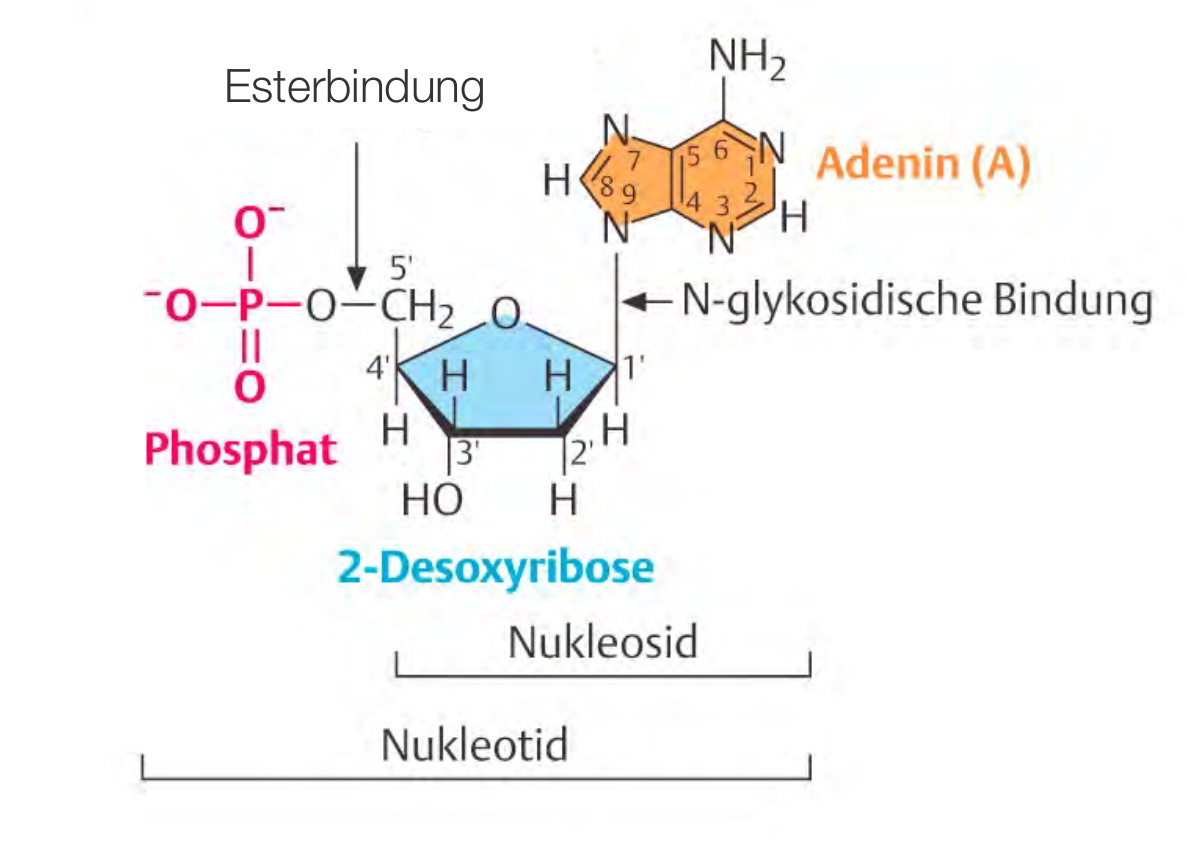
\includegraphics[width=\textwidth]{bilder/nukleotid}
    \caption{}\label{fig:figure4} % TODO Caption
\end{figure}

% TODO Bildverdeckung

\defin{nukleosid}
\defin{nukleotid}

\begin{figure}[H]
    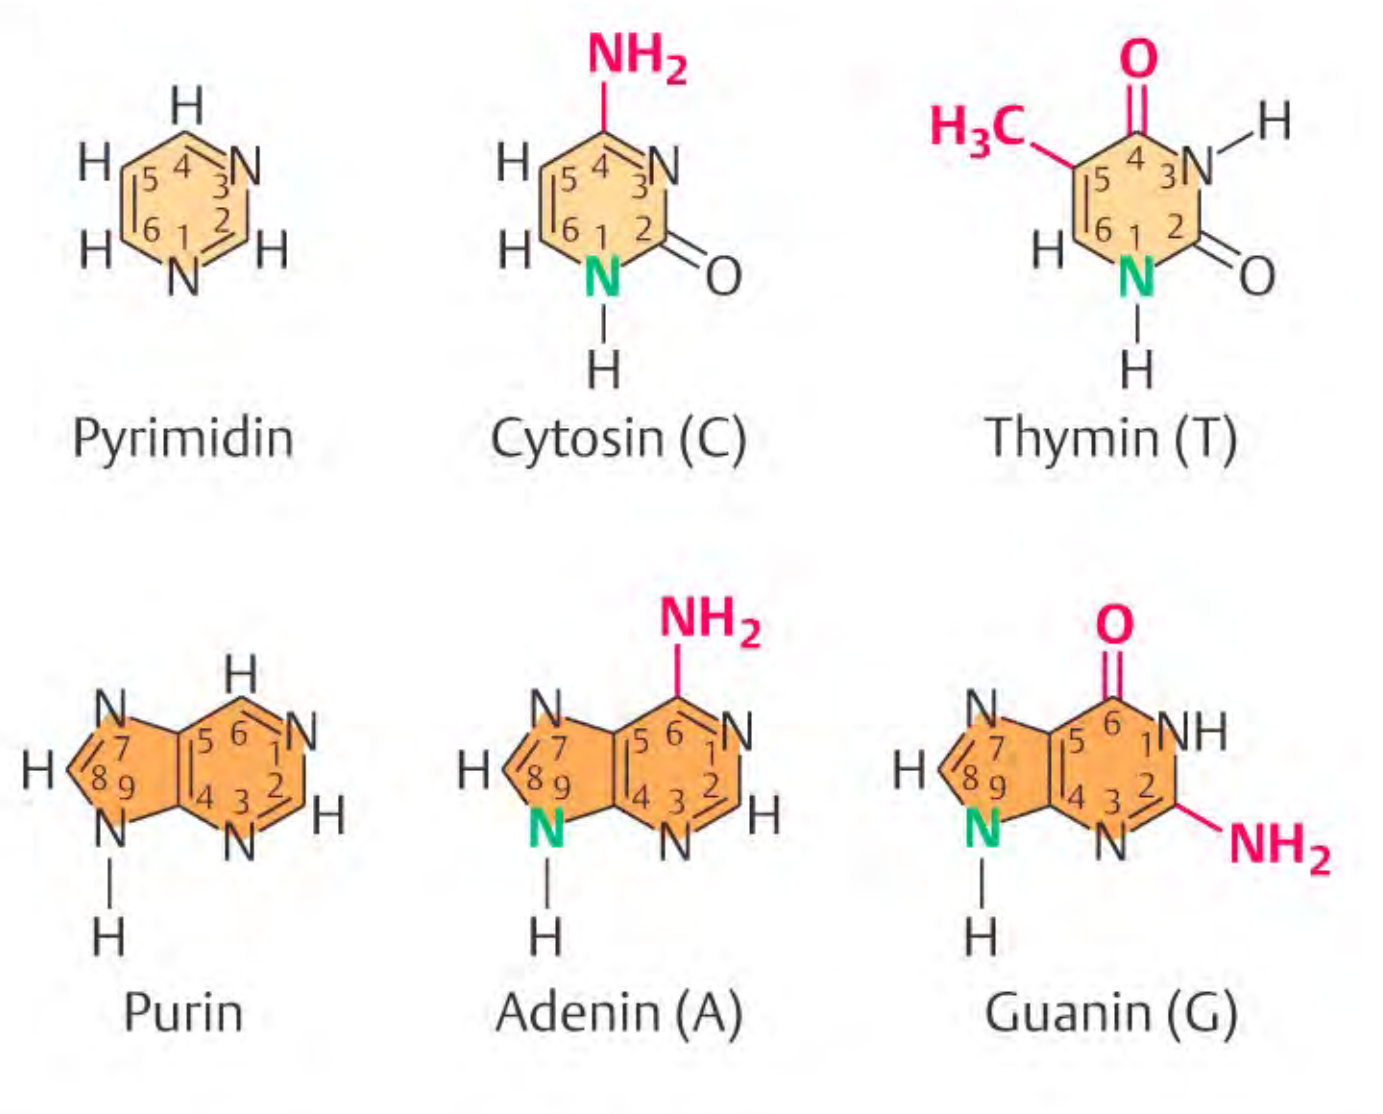
\includegraphics[width=\textwidth]{bilder/basen}
    \caption{}\label{fig:figure3} % TODO Caption
\end{figure}


\defin{pyrimidin}
\defin{purin}

\subsection{Bezeichnungen der Nukleoside}\label{subsec:bezeichnungen-der-nukleoside}

% TODO F 24 - 25

\section{RNA}\label{sec:rna}

% TODO GANZ


% TODO 5’ und 3’ - das freie OH was sol einem das sagen???


\section{Der molekulare Aufbau eines DNA-Strangs}\label{sec:der-molekulare-aufbau-eines-dna-strangs}

% TODO Bild + Inhalt + F 32


\regel{Chargaff}

\section{Röntgenbeugungsmuster der DNA}\label{sec:rontgenbeugungsmuster-der-dna}
% TODO F 30-31

\section{Die molekulare Architektur der DNA-Doppelhelix}\label{sec:die-molekulare-architektur-der-dna-doppelhelix}
% TODO F 33-35
\defin{aform}
\defin{bform}
\defin{zform}

\begin{table}[H]
    \centering
    \rowcolors{1}{rose!10}{white}
    \begin{tabular}{cccc}
        & \textbf{A}& \textbf{B} & \textbf{Z} \\
        Proportion \\
        Vorkommen \\
        \gls{händigkeit} \\
        Helixachse \\
        Bp / Helixdrehung \\
        Gycosylbindung \\
    \end{tabular}\label{tab:table} % TODO fertig aussfüllen
\end{table}

% TODO was bedeutet das alles und muss davon noch was definiert werden?


% TODO insgesamt kontrollieren, ob aus irgendwas Karteikarten erstellt werden sollte und wenn ja wie ich das regele

